%!TEX root = ../main.tex

\section{Введение}

\begin{frame}{Физика процесса}
\begin{block}{Электрический пробой}
    Явление резкого возрастания тока в диэлектрике при приложении электрического напряжения выше критического.
\end{block}
\begin{itemize}
    \item Может возникать в стационарных/переменных/импульсных полях
    \item В ряде случаев связан с образованием тонкого проводящего канала
    \item Может приводить к развитию необратимых повреждений в материале
    \item В твердых телах -- наиболее сложный комплекс механизмов, богатая физика
\end{itemize}
\end{frame}


\begin{frame}{Математическая модель}
\begin{block}{Модель типа диффузной границы}
    Вещество находится в разных фазах. Состояние вещества описывается гладкой функцией $\phi(\vx, t)$ -- фазовым полем.
\end{block}
\begin{itemize}
    \item Фазы: $\phi = 1$ -- неповрежденная среда, $\phi = 0$ -- полностью разрушенная
    \item Зона $\phi \in (0, 1)$ -- диффузная граница
    \item На разрушение среды тратится энергия
    \item Возможно учесть произвольную геометрию раздела фаз
\end{itemize}
\begin{figure}
    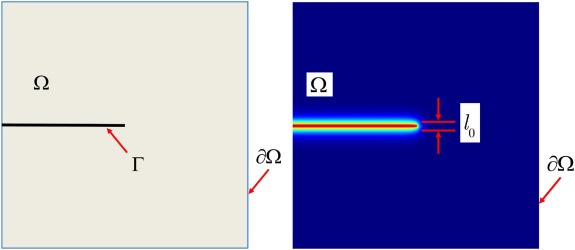
\includegraphics[width=0.5\textwidth]{figures/diffuse_edge.jpg}
\end{figure}
\end{frame}


\begin{frame}{Математическая модель}
%\vspace{-0.3cm}
\begin{block}{Уравнения динамики системы}
    \vspace{-2mm}
    \begin{gather*}
        \Div(\epsilon[\phi] \nabla \Phi) = -\rho_E \\
        \partt{\rho_E} = \Div(\sigma[\phi] \nabla \Phi) \\
        \cfrac{1}{m} \partt{\phi} = -F'( \phi; \| \nabla \Phi \|) + \cfrac{\Gamma}{2} \Delta \phi + \beta \Gamma l^2 \Div \left( \| \nabla \phi \|_2^2 \nabla \phi \right)
    \end{gather*}
    \vspace{-4mm}
\end{block}
\begin{itemize}
    \item $m$, $\Gamma$, $l$, $\beta$ -- параметры модели, константы
\end{itemize}
\end{frame}


\begin{frame}{Математическая модель}
\vspace{-3mm}
\begin{gather*}
    F(\phi; \| \nabla \Phi \|) = -\half \epsilon[\phi] \cdot \| \nabla \Phi \|_2^2 + \cfrac{\Gamma}{l^2} [1 - f(\phi)] \\
    \begin{alignedat}{3}
        \epsilon[\phi] &= \epsilon(\vx, t) &&= \cfrac{\epsilon_0(\vx)}{f(\phi(\vx, t)) + \delta} \\
        \sigma[\phi] &= \sigma(\vx, t) &&= \cfrac{\sigma_0(\vx)}{f(\phi(\vx, t)) + \delta}
    \end{alignedat} \\[2mm]
    f(\phi) = 4 \phi^3 - 3 \phi^4
\end{gather*}
\vspace{-6mm}
\begin{itemize}
    \item $\delta$ -- регуляризующий параметр
    \item $f(\phi)$ -- интерполирующая функция
\end{itemize}
\vspace{1mm}
\parind Модель описана в \cite{zipunova_computational} на основе \cite{pitike_dielectric_breakdown}
\end{frame}


{\nologo
\begin{frame}{Граничные условия}
\begin{columns}
\column{0.6\textwidth}
    \hfill \\[-2mm]
    \hspace*{4mm}
    \begin{tikzpicture}
        \node (image) [anchor=south west, inner sep=0pt] {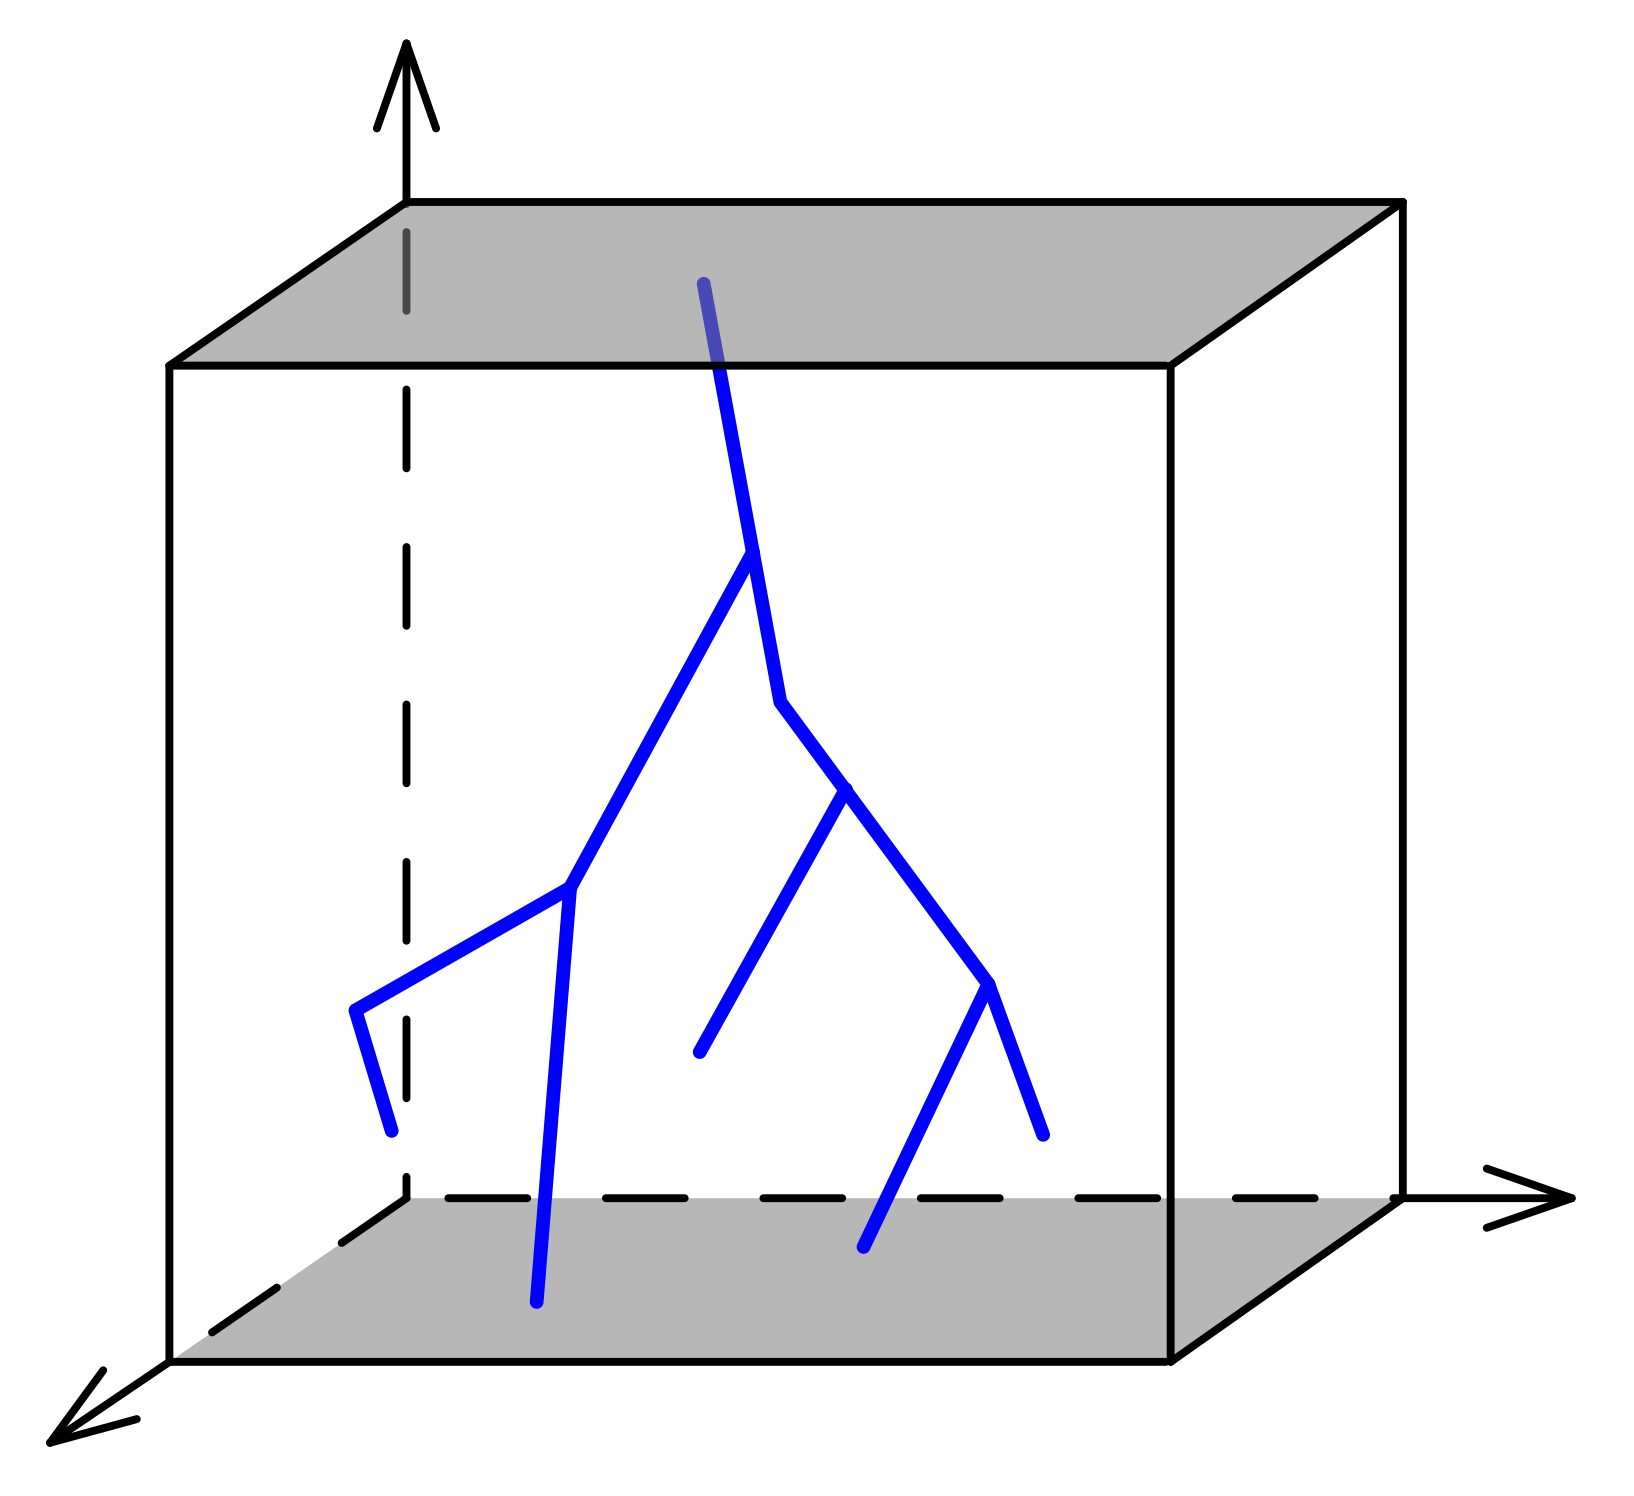
\includegraphics[scale=1.03]{figures/system_scheme.png}};
        \begin{scope}[x={(image.south east)}, y={(image.north west)}]
            \node at (.95, .15) {$x$};
            \node at (.21, .95) {$y$};
            \node at (.03, .1) {$z$};
            \node at (.52, .148) {\small $\Phi = \Phi^+(t); \quad \partvn{\phi} = 0$};
            \node at (.6, .93) {$\Phi = 0; \quad \partvn{\phi} = 0$};
            \node at (.0, .5) {$\partvn{\Phi} = 0;$};
            \node at (.015, .38) {$\phi = 1$};
        \end{scope}
    \end{tikzpicture}
\column{0.4\textwidth}
    \vspace{-5mm}
    \begin{itemize}
        \item Образец диэлектрика \\ в форме параллелепипеда:
    \end{itemize}
    \vspace{2mm}
    \[
        \clOmega = [0, L]_x \times [0, H]_y \times I_z.
    \]
    \vspace{-5mm}
    \begin{itemize}
        \item Зажат между двумя \\ проводящими пластинами \\ под напряжением.
        \item Заряды на обкладках:
    \end{itemize}
    \vspace{-4mm}
    \begin{align*}
        q^+(t) &= -\int\limits_{y = H} \epsilon \cfrac{\partial \Phi}{\partial y} dS; \\
        q^-(t) &= \int\limits_{y = 0} \epsilon \cfrac{\partial \Phi}{\partial y} dS.
    \end{align*}
\end{columns}
\end{frame}
}